\documentclass[12pt,fleqn]{article}\usepackage{../common}
\begin{document}
Kumeleme ile Veri Kurallari Cikartmak

Daha once {\em K-Means Kumeleme Metodu} ile bir veri uzerinde nasil
kumeleme yapacagimizi gorduk. Fakat bazen is dunyasi bu kumelerden akilda
kalacak, tarifsel bazi gozlemlerin ne oldugunu duymak isteyebilir. Mesela
``bayan musterilerimizin cogu saat 5 sonrasi bizden alisveris yapiyor''
gibi bir gozlem. Bu gozlem is sureclerinin iyilestirmesi icin faydali
olabilir, belki yeni bilgi isiginda farkli pazarlama kampanyalari
dusunulur, vs. 

Bu kurallari sistem otomatik olarak bulmalidir, yani ortada bir kesif
durumu olacaktir. Ne bulunanacak? Bilmiyoruz. Veri bilimcilere yapilan bu
tur istekler, bir anlamda, kumsalda oturan bir arkadas grubunda gitar
calmayi bilen arkadasiniza ``abi guzel bir seyler calsana'' diyen kisinin
haline benzer. Kisi guzel bir seyler duymayi istemektedir, ama ne oldugunu
ne o ne de gitar calmayi bilen kisi o anda bilmektedir.

Guzel bir seyler calalim o zaman (!). Tabii verinin uzerinde sadece K-Means
ya da baska bir kumeleme algoritmasi isletmek yeterli olmaz. K-Means'e
mesela ``10 tane kume bul'' denecektir, o da gidip takir takir 10 tane kume
bulacaktir. Fakat bu kumelerin icinde ne vardir? Ilginc hangi tur kurallar
cikartabiliriz? 

Ornek veri olarak {\em Pivotlama} yazisindanki Movielens 1M verisini
kullanacagiz. Ayrica bu verideki posta kodu (zip) ve iskolu (occupation)
veisine README'ye ve bir Internet sitesine [1] danisarak sozel
aciklamalarini koyduk. Boylece sonuclari yorumlamak cok daha kolay olacak. 

\begin{minted}[fontsize=\footnotesize]{python}
import pandas as pd
cols = ['user_id', 'gender', 'age', 'occupation', 'zip']
users = pd.read_csv('../stat_pandas_ratings/users.dat', sep='::', 
        header=None,names=cols)

occup_map = \
{ 0:  "other" or not specified,1:  "academic/educator",
  2:  "artist",3:  "clerical/admin",
  4:  "college/grad student",5:  "customer service",
  6:  "doctor/health care",7:  "executive/managerial",
  8:  "farmer",9:  "homemaker",
  10:  "K-12 student", 11:  "lawyer",
  12:  "programmer",13:  "retired",
  14:  "sales/marketing",15:  "scientist",
  16:  "self-employed",17:  "technician/engineer",
  18:  "tradesman/craftsman",19:  "unemployed",
  20:  "writer"}

zip_map = \
{ 0: 'Northeast', 1: 'NY Area', 2: 'DC', 3: 'Florida', 4: 'Michigan/Ohio', 
  5: 'North', 6: 'Illinois', 7: 'Texas / Arkansas', 8: 'Nevada / Utah', 
  9: 'California / Alaska'}

from sklearn.feature_extraction import DictVectorizer
def one_hot_dataframe(data, cols):
    vec = DictVectorizer()
    mkdict = lambda row: dict((col, row[col]) for col in cols)
    tmp = vec.fit_transform(data[cols].to_dict(outtype='records')).toarray()
    vecData = pd.DataFrame(tmp)
    vecData.columns = vec.get_feature_names()
    vecData.index = data.index
    data = data.drop(cols, axis=1)
    data = data.join(vecData)
    return data

df = users.copy()
df['occupation'] = df.apply(lambda x: occup_map[x['occupation']], axis=1)
df['zip2'] = users['zip'].map(lambda x: int(str(x)[0]))
df['zip2'] = df.apply(lambda x: zip_map[x['zip2']], axis=1)
df = one_hot_dataframe(df,['occupation','gender','zip2'])
df = df.drop(['zip'],axis=1)
df = df.set_index('user_id')
\end{minted}

ZIP kodlari altta gosteriliyor

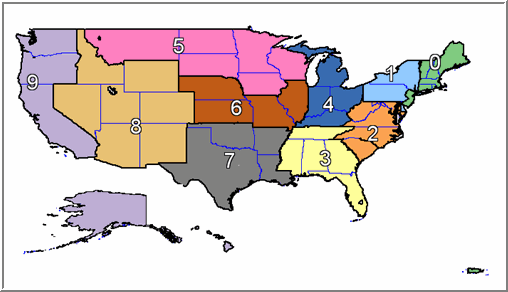
\includegraphics[height=7cm]{zip_code_zones.png}

Simdi hangi film genre'sinin (turunun) kullanici tarafindan kac kez alinmis
oldugunu ozetleyip kullanici verisine bitisik olarak ekleyecegiz. 

\begin{minted}[fontsize=\footnotesize]{python}
cols = ['user_id', 'movie_id', 'rating', 'timestamp']
ratings =  pd.read_csv('../stat_pandas_ratings/ratings.dat', sep='::',
           header=None,names=cols)
cols = ['movie_id', 'title', 'genres']
movies =  pd.read_csv('../stat_pandas_ratings/movies.dat',sep='::',
          header=None,names=cols)

genre_iter = (set(x.split('|')) for x in movies.genres)
genres = sorted(set.union(*genre_iter))
dummies = pd.DataFrame(np.zeros((len(movies), len(genres))), columns=genres)
for i, gen in enumerate(movies.genres):
   dummies.ix[i, gen.split('|')] = 1
movies_windic = movies.join(dummies.add_prefix('Genre_'))
movies_windic = movies_windic.drop(['title','genres'],axis=1)
joined = ratings.merge(movies_windic, left_on='movie_id',right_on='movie_id')
genres = joined.groupby('user_id').sum()
genres = genres.drop(['movie_id','rating','timestamp'],axis=1)
X = pd.merge(df, genres, left_index=True, right_index=True,how='left')
print X.shape
\end{minted}

\begin{verbatim}
(6040, 52)
\end{verbatim}

Veri hazir. Altta bir de kolon tarif dosyasi uretiyoruz, bu birazdan
kullanacagimiz \verb!xgboost! agac yapisinin veri kolon isimlerine
erisebilmesi icin gerekli. Numerik degerler \verb!q!, 1-hot ile
kodlanmis ikisel kolonlar \verb!i! ile isaretleniyor,

\begin{minted}[fontsize=\footnotesize]{python}
fout = open('/tmp/featmap.txt','wb')
for i,col in enumerate(X.columns):
    if  'age'==col: fout.write('%d\t%s\tq\n' % (i,col))
    else: fout.write('%d\t%s\ti\n' % (i,col))    
fout.close()
\end{minted}

Simdi kural cikartmak icin ilk yapmamiz gereken, K-Means yazisinda
gordugumuz gibi, SVD isletmek. Bu daraltilmis boyut uzerinde ardindan
K-Means kumelemesi yapacagiz. SVD'nin kac boyuta indirgemesi gerektigini
once buyukce bir boyuta indirgeyip $s$'e bakarak, daha gerekli ufak boyutu
ona gore ayarlayarak yapiyoruz.

\begin{minted}[fontsize=\footnotesize]{python}
print list(X.columns)
from sklearn.preprocessing import normalize
import scipy.sparse.linalg as slin
import scipy.linalg as lin
import scipy.sparse as sps, numpy.random as rand
rand.seed(0) # tohumu set et svds icinde rasgele islemler var
X2 = sps.csr_matrix(X.fillna(0))
X2 = normalize(X2, norm='l2', axis=0).tocsr()
X2 = normalize(X2, norm='l2', axis=1).tocsr()    
u,s,v=slin.svds(X2,10)
print s
u,s,v=slin.svds(X2,2)
print s
\end{minted}

\begin{verbatim}
['age', 'gender=F', 'gender=M', 'occupation=K-12 student', 'occupation=academic/educator', 'occupation=artist', 'occupation=clerical/admin', 'occupation=college/grad student', 'occupation=customer service', 'occupation=doctor/health care', 'occupation=executive/managerial', 'occupation=farmer', 'occupation=homemaker', 'occupation=lawyer', 'occupation=other', 'occupation=programmer', 'occupation=retired', 'occupation=sales/marketing', 'occupation=scientist', 'occupation=self-employed', 'occupation=technician/engineer', 'occupation=tradesman/craftsman', 'occupation=unemployed', 'occupation=writer', 'zip2=California / Alaska', 'zip2=DC', 'zip2=Florida', 'zip2=Illinois', 'zip2=Michigan/Ohio', 'zip2=NY Area', 'zip2=Nevada / Utah', 'zip2=North', 'zip2=Northeast', 'zip2=Texas / Arkansas', 'Genre_Action', 'Genre_Adventure', 'Genre_Animation', "Genre_Children's", 'Genre_Comedy', 'Genre_Crime', 'Genre_Documentary', 'Genre_Drama', 'Genre_Fantasy', 'Genre_Film-Noir', 'Genre_Horror', 'Genre_Musical', 'Genre_Mystery', 'Genre_Romance', 'Genre_Sci-Fi', 'Genre_Thriller', 'Genre_War', 'Genre_Western']
[ 12.90224699  13.16705714  13.47682441  13.74636749  14.19019079
  14.6403545   14.79911427  15.23097981  16.22546324  36.78813713]
[ 16.22546324  36.78813713]
\end{verbatim}

Goruluyor ki ``enerji'' ilk iki kolonda. Bu sebeple $k=2$ olarak aldik.

Simdi K-Means'e gelelim. Kumelemeyi yapip kume etiketini musteri verisine
bir kolon olarak ekliyoruz. 

\begin{minted}[fontsize=\footnotesize]{python}
n_clusters=6
from sklearn.cluster import KMeans
print u.shape
clf = KMeans(n_clusters=n_clusters,init='k-means++')
clf.fit(u)    
df2 = X.reset_index()
df2['cluster'] = clf.labels_
df2.to_csv('/tmp/customers_clustered.csv',sep=';',index=None)
\end{minted}

\begin{verbatim}
(6040, 2)
\end{verbatim}

Simdi isin en ilginc kismina geldik! Kurallari cikartma zamani.

Kurallari nasil bulacagimizi dusunurken aklimiza ilginc bir fikir
geldi. Kumeleme proseduru kumeleri buldu.. Bundan sonra kurallari bulmak
icin o kumelerin icine bir sekilde bakmak lazim.. Bu nasil yapilacak?
Hangi teknoloji bize ``tarifler'' uretir? Acaba her kume icin o kumedeki
veri noktalarini 1, digerlerini 0 ile isaretlesek, o kumenin tariflerini
bulma isini karar agaci kullanan bir takip edilen (supervised) probleme
ceviremez miyiz ? Tabii burada bir cinlik yapmaya ugrasiyoruz, aslinda
amacimiz ``hic gormedigimiz yeni veri noktalarini'' 1/0 olarak
etiketleyebilmek degil, ki takip edilen yapay ogrenimde amac bu
olurdu. Bizim amacimiz baska: 1/0 ile etiketli veride karar agaci
(ozellikle gradyan destekli karar agaci \verb!xgboost!) kullanmak ve bu
teknolojinin egitim sirasinda ortaya cikardigi karar agaci kurma
mekanizmasindan istifade etmek; cunku ortaya cikan agac yapilarini ``veri
hakkinda baskalarina soylenebilecek ilginc seyler'' olarak kullanabiliriz!

Altta \verb!xgboost! [2] ile bu isi yapiyoruz. 

\begin{minted}[fontsize=\footnotesize]{python}
from sklearn.metrics import roc_curve, auc
from sklearn.cross_validation import train_test_split
import os.path,os,logging,datetime,pytz,re, sys
sys.path.append('%s/Downloads/xgboost/wrapper/' % os.environ['HOME'])
import xgboost as xgb

df3 = pd.read_csv('/tmp/customers_clustered.csv',sep=';',index_col='user_id')
X3 = df3.drop('cluster',axis=1)
print X3.shape

aucs = []
for i in range(n_clusters):
    y = (df3['cluster'] == i).astype(float)    
    X_train, X_test, y_train, y_test = train_test_split(X3, y, test_size=0.10, random_state=0)
    xg_train = xgb.DMatrix(X_train, label=y_train)
    xg_test = xgb.DMatrix(X_test, label=y_test)    
    watchlist = [ (xg_train,'train'), (xg_test, 'test') ]    
    param = {}; 
    num_round = 20
    param['silent'] = 1
    param['eval_metric'] = 'auc'
    param['max_depth'] = 3
    bst = xgb.train(param, xg_train, num_round, watchlist )
    pred = bst.predict(xg_test)
    fpr, tpr, thresholds = roc_curve(y_test, pred)
    roc_auc = auc(fpr, tpr)
    print 'cluster', i, roc_auc, np.sum(y)
    aucs.append(roc_auc)
    bst.dump_model('/tmp/tree-%d.txt' % i,'/tmp/featmap.txt')
print 'mean auc', np.array(aucs).mean()
\end{minted}

\begin{verbatim}
(6040, 52)
cluster 0 0.918416234622 1274.0
cluster 1 0.910995271372 1227.0
cluster 2 0.995317361044 574.0
cluster 3 0.921009290541 1578.0
cluster 4 0.961492309371 895.0
cluster 5 0.988740844631 492.0
mean auc 0.94932855193
\end{verbatim}

Ustte her kume icin bir karar agaci egitiyoruz. Elde edilen AUC kumelemenin
ne kadar basarili oldugunu gormek icin kullanilabilir. Eger kumeler icinde
hicbir oruntu olmasaydi, \verb!xgboost! bu oruntu ile etiket arasinda
hicbir korelasyon bulamazdi. Bulduguna gore durum iyi.

Karar agaclarini analiz etmek icin once her cikti dosyasini teker teker
ziyaret edecegiz, ve tum dugum (node) ve dallar (branches) bilgilerini
okuyacagiz. Daha sonra ozyineli (recursive) bir prosedur ile her agacin en
ust yani \verb!0! dugumunden baslayip tum dallarini ziyaret edecegiz, en
alt noktaya geldigimizde ebeyne (parent) dogru elimizde tuttugumuz
isaretleri takip ede ede en ust noktaya, yani \verb!0! dugumune gidecegiz
bu ``yolu'' bir kenara yazagiz, cunku bu yol bir kurali temsil etmektedir.

Bir yolu ortaya cikardiktan sonra bir sukseli hareket daha yapacagiz,
kurali alip onu direk Pandas dilimleme (slicing) kurali haline getirecegiz,
ve bu kuralin kac veri satirina tekabul ettigini aninda gorecegiz. Hatta
bir dilim uzerinde ek istedigimiz istatistigi de otomatik olarak
hesaplattirabiliriz! 

\inputminted[fontsize=\footnotesize]{python}{clusters.py}

\begin{minted}[fontsize=\footnotesize]{python}
!python clusters.py
\end{minted}

\begin{verbatim}
original dataset 6040

('zip2=Texas / Arkansas', 'no')
('occupation=programmer', 'no')
("Genre_Children's", 'yes')

count 675

('age<9.5', 'no')
('zip2=NY Area', 'no')
('Genre_Animation', 'yes')

count 790

('occupation=academic/educator', 'no')
('zip2=California / Alaska', 'yes')
('occupation=executive/managerial', 'no')

count 1216

('occupation=academic/educator', 'no')
('zip2=California / Alaska', 'no')
('occupation=other', 'yes')

count 529

('age<40', 'yes')
('zip2=NY Area', 'no')
('zip2=California / Alaska', 'yes')

count 1128

('age<40', 'yes')
('zip2=NY Area', 'no')
('zip2=California / Alaska', 'no')

count 2984

('age<9.5', 'no')
('Genre_Fantasy', 'yes')
('occupation=academic/educator', 'no')

count 992

('occupation=scientist', 'no')
('Genre_Animation', 'yes')
('occupation=other', 'no')

count 764

('zip2=Illinois', 'no')
('age<9.5', 'no')
('Genre_Horror', 'yes')

count 663

('occupation=customer service', 'no')
('occupation=clerical/admin', 'no')
('age<21.5', 'yes')

count 1289

('zip2=NY Area', 'no')
('zip2=Northeast', 'yes')
('occupation=doctor/health care', 'no')

count 637

('zip2=NY Area', 'no')
('zip2=Northeast', 'no')
('zip2=California / Alaska', 'yes')

count 1468

('age<40', 'yes')
('zip2=NY Area', 'no')
('occupation=executive/managerial', 'yes')

count 410

('age<40', 'yes')
('zip2=NY Area', 'no')
('occupation=executive/managerial', 'no')

count 3702

('occupation=customer service', 'no')
('occupation=K-12 student', 'no')
('Genre_Mystery', 'yes')

count 918

('occupation=college/grad student', 'no')
('Genre_Fantasy', 'yes')
('Genre_Western', 'no')

count 490

('Genre_Film-Noir', 'no')
('Genre_Fantasy', 'yes')

count 491

('occupation=unemployed', 'no')
('Genre_Documentary', 'no')
('Genre_Fantasy', 'yes')

count 806

('occupation=farmer', 'no')
('occupation=academic/educator', 'no')
('occupation=other', 'yes')

count 711

('occupation=technician/engineer', 'no')
('occupation=college/grad student', 'no')
('occupation=executive/managerial', 'yes')

count 679

('occupation=executive/managerial', 'no')
('occupation=other', 'yes')
('zip2=California / Alaska', 'no')

count 529

('occupation=executive/managerial', 'no')
('occupation=other', 'no')
('occupation=academic/educator', 'yes')

count 528

('occupation=executive/managerial', 'no')
('occupation=other', 'no')
('occupation=academic/educator', 'yes')

count 528

('occupation=executive/managerial', 'no')
('zip2=California / Alaska', 'yes')
('occupation=academic/educator', 'no')

count 1216

('occupation=executive/managerial', 'no')
('zip2=California / Alaska', 'no')
('zip2=NY Area', 'yes')

count 556

('zip2=NY Area', 'no')
('zip2=California / Alaska', 'yes')
('occupation=academic/educator', 'no')

count 1357

('zip2=NY Area', 'no')
('zip2=California / Alaska', 'no')
('zip2=Northeast', 'yes')

count 662

('Genre_Crime', 'yes')
('occupation=academic/educator', 'no')
('occupation=other', 'no')

count 440

('zip2=NY Area', 'yes')
('occupation=academic/educator', 'no')
('occupation=executive/managerial', 'no')

count 499

('zip2=NY Area', 'no')
('age<53', 'yes')
('zip2=California / Alaska', 'yes')

count 1372

('zip2=NY Area', 'no')
('age<53', 'yes')
('zip2=California / Alaska', 'no')

count 3669

('zip2=NY Area', 'no')
('zip2=Northeast', 'no')
('occupation=technician/engineer', 'yes')

count 422

('Genre_Fantasy', 'yes')
('zip2=California / Alaska', 'no')
('zip2=NY Area', 'no')

count 714

('Genre_Musical', 'yes')
('zip2=California / Alaska', 'no')
('occupation=executive/managerial', 'no')

count 708
\end{verbatim}

Kurallar ortaya cikti. Ilginc bir tanesi mesela 

\begin{verbatim}
('age<9.5', 'no')
('zip2=NY Area', 'no')
('Genre_Animation', 'yes')

count 790
\end{verbatim}

Yani animasyon turu filmler seven bir grup insan (onemli bir grup, cunku
bir cok satira tekabul ediyor) \verb!9.5! yas uzerindeler (ve New York'ta
yasamiyorlar, ama bu o kadar onemli olmayabilir). Burada bir noktaya
aciklik getirelim, Movielens 1M verisinde yas, 1,18,25 gibi degerler ve bu
degerler aslinda belli araliklara tekabul eden kodlar. Mesela 1 kodu 18
yasinin alti demekmis. Yani eger karar agaci 9.5'ten buyuk olmali kuralini
bulduysa (cunku 9.5'ten kucuk kurali yaninda 'no' yaziyor, demek ki tersi
gecerli), o zaman bulunan esik $\ge 18$ demektir.

Hakikaten de 

\begin{minted}[fontsize=\footnotesize]{python}
import pandas as pd
dff = pd.read_csv('/tmp/customers_clustered.csv',sep=';',index_col='user_id')
print len(dff)
\end{minted}

\begin{verbatim}
6040
\end{verbatim}

\begin{minted}[fontsize=\footnotesize]{python}
print len( dff[\
(dff['Genre_Animation'] == 1) & \
(dff['age'] >= 18 ) ] )
\end{minted}

\begin{verbatim}
874
\end{verbatim}

Bir kural kesfedildi! Bu bulguyu sosyal olarak dusunelim, ilginc aslinda,
yani animasyonun kucuk cocuklar tarafindan daha cok sevilecegini
dusunurduk, ama veri boyle demiyor. Cocuklari kontrol edelim,

\begin{minted}[fontsize=\footnotesize]{python}
print len( dff[\
(dff['Genre_Animation'] == 1) & \
(dff['age'] < 18 ) ] )
\end{minted}

\begin{verbatim}
21
\end{verbatim}

Cok az. Buyukler animasyonu daha cok seviyormus demek ki.  Iste bu bir
bulgu. Veri madenciligi, kumeleme sayesinde bunu bulmus olduk.

Akla gelebilecek diger bazi kurallari da kontrol edebiliriz, ``niye yok''
diye aklimiza takildi mesela, ``erkekler aksiyon sever'' gibi. Bu kural
bulunmamisti... Acaba kodumuzda bir yanlislik mi vardi? Veriye bakiyoruz,

\begin{minted}[fontsize=\footnotesize]{python}
print 'Erkek', len( dff[(dff['Genre_Action'] == 1) & (dff['gender=M'] == 1 ) ] ),\
      'Bayan', len( dff[(dff['Genre_Action'] == 1) & (dff['gender=F'] == 1 ) ] )
\end{minted}

\begin{verbatim}
Erkek 41 Bayan 51
\end{verbatim}

Bunlar muthis dusuk rakamlar. Kural bulunmamis cunku ortada bir kalip yok.

[1] \url{http://www.zipboundary.com/zipcode_faqs.html}

[2] \url{http://sayilarvekuramlar.blogspot.de/2014/09/gradient-boosted-regression-trees-gbrt.html}

\end{document}
